
% v2-acmsmall-sample.tex, dated March 6 2012
% This is a sample file for ACM small trim journals
%
% Compilation using 'acmsmall.cls' - version 1.3 (March 2012), Aptara Inc.
% (c) 2010 Association for Computing Machinery (ACM)
%
% Questions/Suggestions/Feedback should be addressed to => "acmtexsupport@aptaracorp.com".
% Users can also go through the FAQs available on the journal's submission webpage.
%
% Steps to compile: latex, bibtex, latex latex
%
% For tracking purposes => this is v1.3 - March 2012
\documentclass[prodmode,acmtecs]{acmsmall} % Aptara syntax
\usepackage[spanish,polish]{babel}
\usepackage[T1]{fontenc}
\usepackage{fancyvrb}
\usepackage{graphicx,hyperref}
\newcommand\cutout[1]{}


\usepackage[table]{xcolor}
\usepackage[utf8]{inputenc}
\usepackage[parfill]{parskip}
\usepackage{tabulary}
\PassOptionsToPackage{hyphens}{url}
\usepackage{hyperref}    
\usepackage[capitalize]{cleveref}


% Metadata Information
% !!! TODO: SET THESE VALUES !!!
\acmVolume{0}
\acmNumber{0}
\acmArticle{CFP}
\acmYear{0}
\acmMonth{0}

\newcounter{colstart}
\setcounter{page}{4}

\RecustomVerbatimCommand{\VerbatimInput}{VerbatimInput}%
{
%fontsize=\footnotesize,
fontfamily=\rmdefault
}


\newcommand{\UnderscoreCommands}{%\do\verbatiminput%
\do\citeNP \do\citeA \do\citeANP \do\citeN \do\shortcite%
\do\shortciteNP \do\shortciteA \do\shortciteANP \do\shortciteN%
\do\citeyear \do\citeyearNP%
}

\usepackage[strings]{underscore}



% Document starts
\begin{document}


\setcounter{colstart}{\thepage}

\acmArticle{CFP}
\title{{\huge\sc SIGLOG Monthly 255}

 November 2024}\author{ELLI ANASTASIADI\affil{Uppsala University, SE}\vspace*{-2.6cm}\begin{flushright}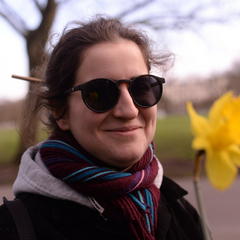
\includegraphics[width=30mm]{elli_anastasiadi.png}\end{flushright}}\begin{abstract}November 2024 edition of SIGLOG Monthly, featuring deadlines, calls and community announcements.
\end{abstract}


\maketitlee

\href{https://lics.siglog.org/newsletters/}{Past Issues}
 - 
\href{https://lics.siglog.org/newsletters/inst.html}{How to submit an announcement}
\section{Table of Contents}\begin{itemize}\item DEADLINES (\cref{deadlines}) 
 
\item CALLS 
 
\begin{itemize}\item CiE 2025 (CALL FOR PAPERS) (\cref{CiE2025})
\item CAV 2025 (CALL FOR PAPERS) (\cref{CAV2025})
\item FSCD 2025 (CALL FOR PAPERS) (\cref{FSCD2025})
\item DEON 2025 (CALL FOR PAPERS) (\cref{DEON2025})
\item FSCD 2025 WORKSHOPS (CALL FOR WORKSHOPS) (\cref{FSCD2025WORKSHOPS})
\end{itemize} 
\item JOB ANNOUNCEMENTS 
 
\begin{itemize}\item University Assistant (Prae-Doc) (\cref{UniversityAssistantPraeDoc})
\end{itemize} 
\end{itemize}\section{Deadlines}\label{deadlines}\rowcolors{1}{white}{gray!25}\begin{tabulary}{\linewidth}{LL}University Assistant (Prae-Doc):  & Nov 28, 2024 (Application deadline) \\
LICS 2025 WORKSHOPS:  & Nov 30, 2024 (Submission of workshop proposals) \\
FSCD 2025 WORKSHOPS:  & Dec 12, 2024 (Workshop proposal) \\
LICS 2025:  & Jan 16, 2025 (Abstract), Jan 23, 2025 (Full Papers) \\
CiE 2025:  & Jan 26, 2025 (Abstract), Feb 02, 2025 (Full paper) \\
CAV 2025:  & Jan 31, 2025 (Full paper) \\
FSCD 2025:  & Feb 10, 2025 (Abstract), Feb 17, 2025 (Full paper) \\
DEON 2025:  & Mar 01, 2025 (Abstract  deadline), Mar 08, 2025 (Paper  deadline) \\
\end{tabulary}
\section{CiE 2025: Computability in Europe 2025 }\label{CiE2025}  Crossroads of Computability and Logic: Insights, Inspirations, and Innovations\\ 
  Lisbon, Portugal, July 14-18, 2025\\ 
  \href{https://bit.ly/CIE2025}{https://bit.ly/CIE2025}\\ 
CALL FOR PAPERS 

\begin{itemize}\item  IMPORTANT DATES (AOE): 
 
\rowcolors{1}{white}{gray!25}\begin{tabulary}{\linewidth}{LL}Abstract submission:  & Jan 26, 2025 \\
Full paper submission:  & Feb 02, 2025 \\
Notification of acceptance:  & Apr 06, 2025 \\
Final versions due:  & Apr 13, 2025 \\
Informal presentations submission:  & Apr 22, 2025 \\
Early registration before:  & May 06, 2025 \\
Conference:  & July 14-18, 2025 \\
\end{tabulary}
 
  The notifications of acceptance for informal presentations will be sent a few days after submission. 
 
\item  GENERAL INFORMATION 
 
  CiE 2025 will be the 21st conference organized by CiE (Computability in Europe). CiE is a European association of mathematicians, logicians, computer scientists, philosophers, physicists and others interested in new developments in computability and their underlying significance for the real world. 
 
\item  TUTORIAL SPEAKERS 
 
\begin{itemize}\item  Maria Paola Bonacina (University of Verona)
\item  Igor Carboni Oliveira (University of Warwick)
\end{itemize} 
\item  INVITED SPEAKERS 
 
\begin{itemize}\item  Ugo Dal Lago (University of Bologna)
\item  Daniel Graça (University of Algarve)
\item  Ekaterina Komendantskaya (University of Southampton)
\item  Ng Keng Meng (Nanyang Technological University)
\item  Paulo Oliva (Queen Mary University of London)
\item  Ana Sokolova (University of Salzburg)
\end{itemize} 
\item  SPECIAL SESSIONS 
 
  There will be 6 special sessions, details will be announced soon. 
 
\item  CONFERENCE TOPICS 
 
  The CiE conferences serve as an interdisciplinary forum for research in all aspects of computability, foundations of computer science, logic, and theoretical computer science, as well as the interplay of these areas with practical issues in computer science and with other disciplines such as biology, mathematics, philosophy, or physics. 
 
\item  PAPER SUBMISSION 
 
 The Program Committee cordially invites all researchers, European and non-European, to submit their papers in all areas related to the above for presentation at the conference and inclusion in the proceedings of CiE 2025 at \href{https://easychair.org/my/conference?conf=cie2025}{https://easychair.org/my/conference?conf=cie2025}. 
 
\item  CONFERENCE PROCEEDINGS 
 
  Papers submitted to the conference proceedings should represent original work, not simultaneously submitted to another journal or conference with formal proceedings. The Program Committee will rigorously review and select submitted papers. Accepted papers will be published as a proceedings volume in the Lecture Notes in Computer Science (LNCS) series from Springer-Verlag. Papers to be considered in the conferences proceedings must be submitted in PDF format, using the LNCS style (available at \href{https://www.springer.com/gp/}{https://www.springer.com/gp/}) and must have a maximum of 15 pages, including references but excluding a possible appendix in which one can include proofs and other additional material. Papers building bridges between different parts of the research community are particularly welcome. 
 
\item  INFORMAL PRESENTATIONS 
 
  Continuing the tradition of past CiE conferences, we invite researchers to present informal presentations of their recent work. A proposal for an informal presentation must be submitted via our submission link: \href{https://easychair.org/my/}{https://easychair.org/my/}, using the LNCS style file (available at \href{https://www.springer.com/gp/}{https://www.springer.com/gp/}), and be 1 page long; a brief description of the results suffices and an abstract is not required. Informal presentations will not be published in the LNCS conference proceedings. Results presented as informal presentations at CiE 2025 may appear or may have appeared in other conferences with formal proceedings and/or in journals. 
 
\item  WOMEN IN COMPUTABILITY 
 
  We intend to run the Women in Computability program as in previous CiEs, details will be announced in due course. 
 
\item  HOSTED BY 
 
  The event will be held in the Faculdade de Ciências buildings located at University of Lisbon. 
 
\end{itemize}\section{CAV 2025: 37th International Conference on Computer-Aided Verification}\label{CAV2025}  July 21-25, 2025, Zagreb, Croatia\\ 
  \href{https://conferences.i-cav.org/2025/cfp/}{https://conferences.i-cav.org/2025/cfp/}\\ 
CALL FOR PAPERS 

\begin{itemize}\item  CONFERENCE 
 
  CAV 2025 is the 37th in a series dedicated to the advancement of the theory and practice of computer-aided formal analysis methods for hardware and software systems. The conference covers the spectrum from theoretical results to concrete applications, with an emphasis on practical verification tools and the algorithms and techniques that are needed for their implementation. CAV considers it vital to continue spurring advances in hardware and software verification while expanding to new domains such as machine learning, autonomous systems, and computer security. The proceedings of the conference will be published in the Springer-Verlag Lecture Notes in Computer Science series. A selection of papers is expected to be invited to a special issue of Formal Methods in System Design and the Journal of the ACM. 
 
\item  IMPORTANT DATES (AoE) 
 
\rowcolors{1}{white}{gray!25}\begin{tabulary}{\linewidth}{LL}Full paper submission:  & Jan 31, 2025 \\
Author Response Period:  & March 11 - 14, 2025 \\
Author notification:  & Apr 02, 2025 \\
Main Conference:  & July 21-25, 2025 \\
\end{tabulary}
 
\item  TOPICS \& SUBMISSION 
 
  For a full list of topic and submission instructions please check \href{https://conferences.i-cav.org/2025/cfp/}{https://conferences.i-cav.org/2025/cfp/} 
 
\item  CAV AWARD 
 
  The CAV award is given annually at the CAV conference for fundamental contributions to the field of Computer-Aided Verification.  
 
CAV Award Nomination deadline: TBA 
 
  Nominations should include a proposed citation (up to 25 words), a succinct (100-250 words) description of the contribution(s), and a detailed statement to justify the nomination. The cited contribution(s) must have been made not more recently than five years ago and not over twenty five years ago. In addition, the contribution(s) should not yet have received recognition via a major award, such as the ACM Turing or Kanellakis Awards. The nominee may have received such an award for other contributions. For previous winners of the award, please see the main CAV award page: \href{https://i-cav.org/cav-award/}{https://i-cav.org/cav-award/}.  Nominations should be submitted by e-mail to a member of the committee. For details, please see \href{https://conferences.i-cav.org/2025/award/}{https://conferences.i-cav.org/2025/award/}. 
 
\item  CONTACT (CONFERENCE CO-CHAIRS) 
 
  For any questions please contact the PC chairs: 
 
\begin{itemize}\item  Ruzica Piskac (ruzica.piskac at yale.edu)    
\item  Zvonimir Rakamaric (zrakamar at gmail.com)
\end{itemize} 
\end{itemize}\section{FSCD 2025:  Tenth International Conference on Formal Structures for Computation and Deduction}\label{FSCD2025}  14-20 July 2025, Birmingham, UK\\ 
  \href{https://fscd-conference.org/2025/}{https://fscd-conference.org/2025/}\\ 
CALL FOR PAPERS 

\begin{itemize}\item  FSCD (\href{https://fscd-conference.org/}{https://fscd-conference.org/}) covers all aspects of formal structures for computation and deduction, from theoretical foundations to applications. Building on two communities, RTA (Rewriting Techniques and Applications) and TLCA (Typed Lambda Calculi and Applications), FSCD embraces their core topics and broadens their scope to closely related areas in logic, models of computation, semantics and verification in new challenging areas.                    
 
\item  IMPORTANT DATES 
 
  All deadlines are midnight anywhere-on-earth (AoE); late submissions will not be considered. 
 
\rowcolors{1}{white}{gray!25}\begin{tabulary}{\linewidth}{LL}Abstract submission:  & Feb 10, 2025 \\
Full paper submission:  & Feb 17, 2025 \\
Rebuttal:  & April 7-11, 2025 \\
Notification:  & Apr 30, 2025 \\
Final version:  & May 14, 2025 \\
\end{tabulary}
 
  For a full list of topics please check \href{https://fscd2025.github.io/cfp.htm}{https://fscd2025.github.io/cfp.htm} 
 
\item  PUBLICATION 
 
  The proceedings will be published as an electronic volume in the Leibniz International Proceedings in Informatics (LIPIcs) of Schloss Dagstuhl. All LIPIcs proceedings are open access. 
 
\item  SPECIAL ISSUE 
 
  There will be a special issue of Logical Methods in Computer Science of selected papers. More details will be provided later. 
 
\item  SUBMISSION GUIDELINES 
 
  The submission site is: \href{https://easychair.org/conferences/?conf=fscd2025}{https://easychair.org/conferences/?conf=fscd2025} . Submissions must be formatted using the LIPIcs style files (\href{https://submission.dagstuhl.de/series/details/5#author}{https://submission.dagstuhl.de/series/details/5\#author}) and submitted via EasyChair. 
 
\item  Submissions can be made in two categories: regular research papers and system descriptions. Please indicate in the submission page in Easychair and in the first page of the paper in which category you are submitting. Regular research papers are limited to 15 pages, excluding references and appendices. They must present original research which is unpublished and not submitted elsewhere. System descriptions are limited to 15 pages, excluding references. Shorter papers are welcome and will be given equal consideration. A system description must present new software tools, or significantly new versions of such tools, in which FSCD topics play an important role. An archive of the code with instructions on how to install and run the tool must be submitted. In addition, a webpage where the system can be experimented with should be provided. 
 
\item  One author of each accepted paper is expected to register and present the work in person at the conference. In case that this is not possible for some unforeseen reason, online presentation will be arranged, but in person registration will still be required. 
 
\item  BEST PAPER AWARD BY JUNIOR RESEARCHERS 
 
  The programme committee will select a paper in which at least one author is a junior researcher, i.e. either a student or whose PhD award date is less than three years from the first day of the meeting. When submitting the paper, other authors should declare to the PC Chair that at least 50% of contribution is made by the junior researcher(s). 
 
\item  PROGRAMME COMMITTEE CHAIR 
 
\begin{itemize}\item Maribel Fernandez, King's College London, UK Email: fscd2025@easychair.org
\end{itemize} 
\item  CONFERENCE AND LOCAL WORKSHOPS CHAIRS 
 
\begin{itemize}\item  Paul Blain Levy, University of Birmingham, UK
\item  Anupam Das, University of Birmingham, UK
\end{itemize} 
\end{itemize}\section{DEON 2025: 17th International Conference on Deontic Logic and Normative Systems}\label{DEON2025}  30 June – 3 July 2025\\ 
  TU Wien, Vienna, Austria\\ 
CALL FOR PAPERS 

\begin{itemize}\item  The biennial International Conference on Deontic Logic and Normative Systems (DEON) conference series aims at bringing together researchers interested in the formal study of normative concepts, normative reasoning, and normative systems using methods from computer science, artificial intelligence, philosophy, linguistics, mathematics, and law. 
 
\item  IMPORTANT DATES 
 
\rowcolors{1}{white}{gray!25}\begin{tabulary}{\linewidth}{LL}Abstract submission deadline:  & Mar 01, 2025 \\
Paper submission deadline:  & Mar 08, 2025 \\
\end{tabulary}
 
  Please submit electronically using the EasyChair submission page. For more information, please visit \href{https://sites.google.com/view/deon-2025/home}{https://sites.google.com/view/deon-2025/home} 
 
\end{itemize}\section{FSCD 2025 WORKSHOPS}\label{FSCD2025WORKSHOPS}  14-20 July 2025, Birmingham, UK\\ 
  \href{https://fscd-conference.org/2025/}{https://fscd-conference.org/2025/}                       \\ 
CALL FOR WORKSHOPS 

\begin{itemize}\item  IMPORTANT DATES 
 
  All deadlines are midnight anywhere-on-earth (AoE). 
 
\rowcolors{1}{white}{gray!25}\begin{tabulary}{\linewidth}{LL}Workshop proposal:  & Dec 12, 2024 \\
Notification:  & Late January 2025 \\
Workshop programmes:  & May 31, 2025 \\
FSCD 2025 Workshops:  & July 14 and 19-20, 2025 \\
\end{tabulary}
 
\item  OVERVIEW 
 
  FSCD 2025 will take place in Birmingham from 14th to 20th July. We invite proposals for workshops on topics of interest to the FSCD community. 
 
\item  Proposals should include: 
 
\begin{itemize}\item  Workshop's name and URL if already available or from previous years.
\item  A short scientific summary and justification of the proposed topic; this should include a discussion of the particular benefits of any topic related to FSCD.
\item  A list of workshop organisers with contact information. 
\item  Potential invited speakers (please specify expected number and, if possible, tentative names)
\item  Procedures for selecting presentations (if you plan a call for contributed talks or papers followed by a selection procedure, the submission date should be scheduled after the FSCD notification date, while the notification should take place before the early registration deadline).
\item  Plans for publication, if any (e.g. proceeding, journal special issue, etc.)
\item  Proposed format and agenda (e.g. paper presentations, tutorials, demo sessions).
\item  The proposed duration (1 day or 2 days).
\item  Expected number of participants, providing some data on previous years, if the workshop has already been organised in the past.
\item  Any other relevant information and special wishes regarding the schedule (e.g. specific dates, workshops that should (not) be planned on the same day).
\end{itemize} 
\item  LOCAL SUPPORT 
 
  The conference organisers will provide a room, internet connection, coffee breaks, lunches and help with some local organisation. 
 
\item  SUBMISSION 
 
  Proposals must be submitted as a PDF ofat most three pages, not including references by email to: fscd2025@gmail.com . The workshop committee will determine the final list of accepted workshops based on thematic pertinence and time/space availability. 
 
\item  WORKSHOP COMMITTEE 
 
\begin{itemize}\item  Paul Blain Levy (University of Birmingham, UK)
\item  Anupam Das (University of Birmingham, UK)
\item  Cynthia Kop (Radboud University Nijmegen, Netherlands)
\end{itemize} 
\end{itemize}\section{University Assistant (Prae-Doc): TU Wien, Faculty of Informatics, Vienna}\label{UniversityAssistantPraeDoc}JOB ANNOUNCEMENT 

\begin{itemize}\item  At the Institute of Logic and Computation, Research Unit Theory and Logic, Cluster of Excellence “Bilateral AI” . Project “AI Alignment and Dialogues” under the supervision of Kees van Berkel. 40 hours/week, limited to four years, estimated starting date is December 2024 / January 2025 . Details: \href{https://jobs.tuwien.ac.at/Job/241947}{https://jobs.tuwien.ac.at/Job/241947} 
 
Application deadline: Nov 28, 2024 
 
\end{itemize}


\bigskip Links: \href{http://siglog.org/}{SIGLOG website}, \href{https://lics.siglog.org}{LICS website}, \href{https://lics.siglog.org/newsletters/}{SIGLOG Monthly}\end{document}